\section{Introduction}
Tracking is a fundamental task in any video application requiring some degree of reasoning about objects of interest, as it allows to establish object correspondences between frames~\cite{makovski2008visual}. 
It finds use in a wide range of scenarios such as automatic surveillance, vehicle navigation, video labelling, human-computer interaction and activity recognition.
Given the location of an arbitrary target of interest in the first frame of a video, the aim of \emph{visual object tracking} is to estimate its position in all the subsequent frames with the best possible accuracy~\cite{smeulders2014visual}.

\begin{figure}[t]
\centering
\setlength{\tabcolsep}{0.25ex}

\begin{tabular}
{ccc ccccc}
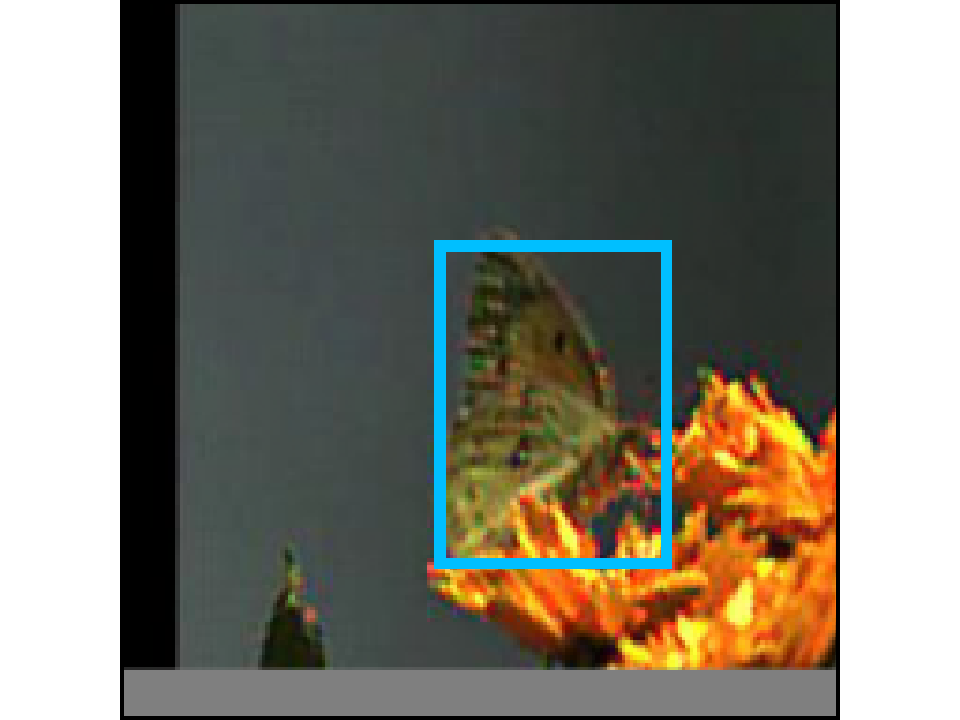
\includegraphics[trim={2cm 0cm 2cm 0cm},clip,width = 0.61in]{img/snapshots/init/00011}
&&&
&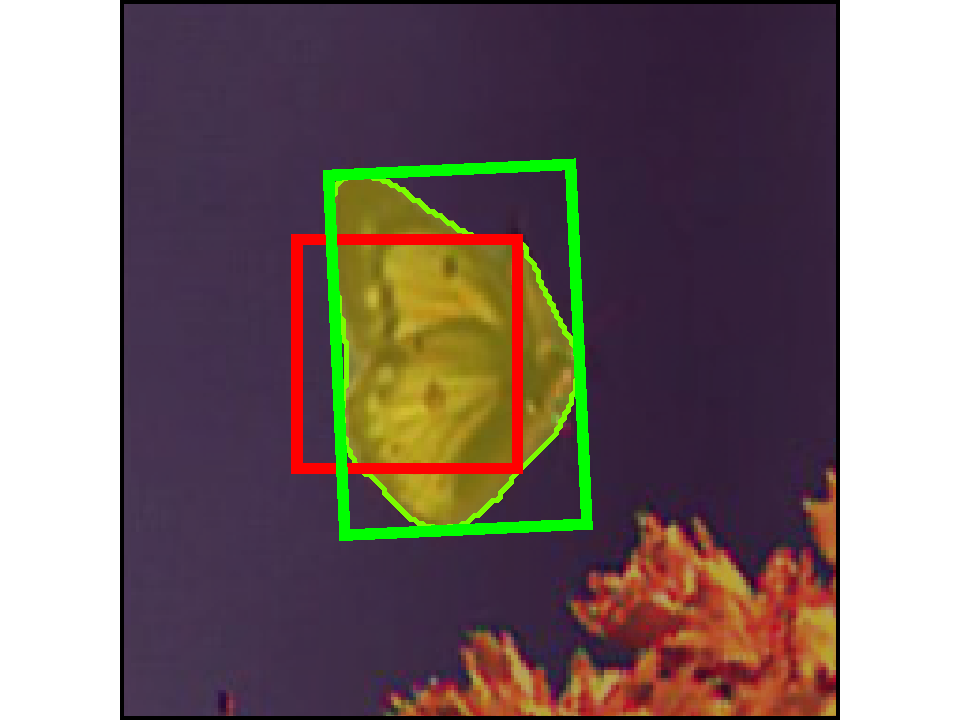
\includegraphics[trim={2cm 0cm 2cm 0cm},clip,width = 0.61in]{img/snapshots/eco_uspblackedge/03073}
& 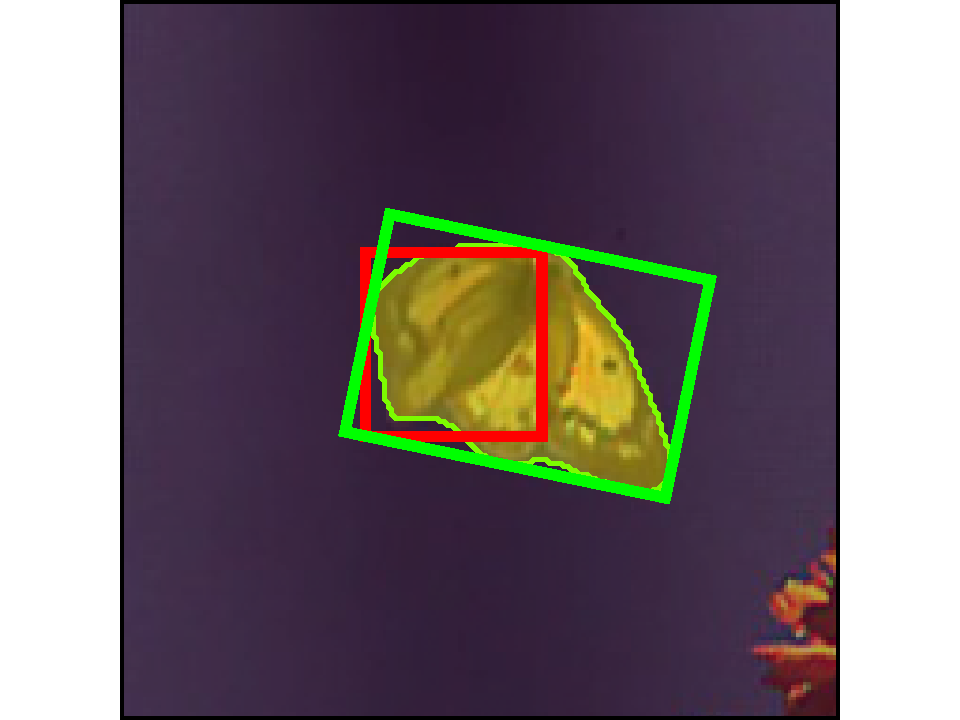
\includegraphics[trim={2cm 0cm 2cm 0cm},clip,width = 0.61in]{img/snapshots/eco_uspblackedge/03108}
& 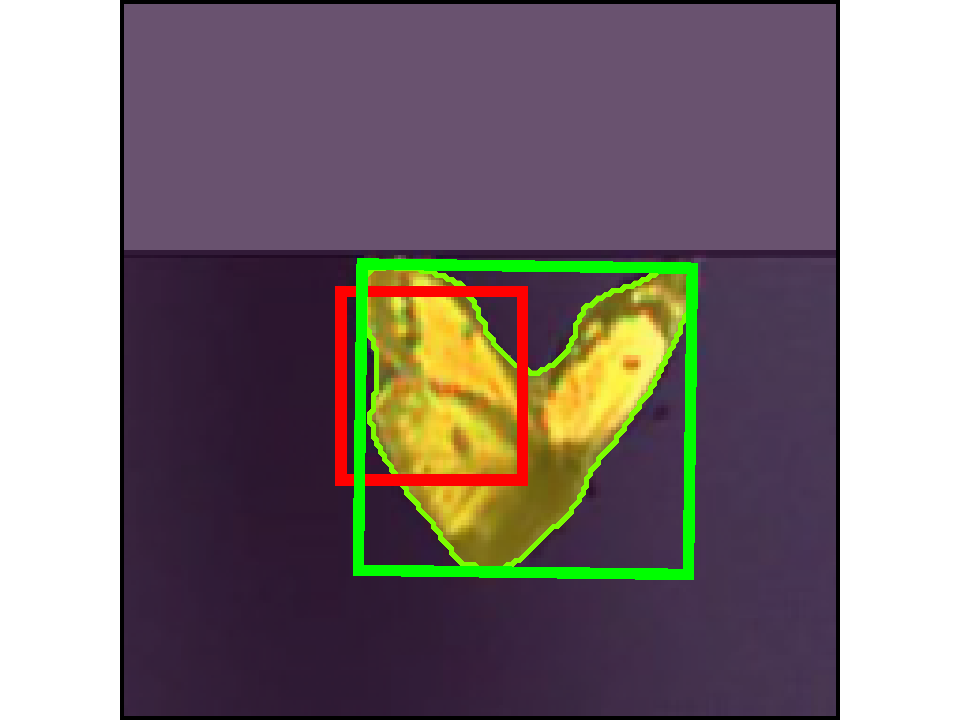
\includegraphics[trim={2cm 0cm 2cm 0cm},clip,width = 0.61in]{img/snapshots/eco_uspblackedge/03143}
& 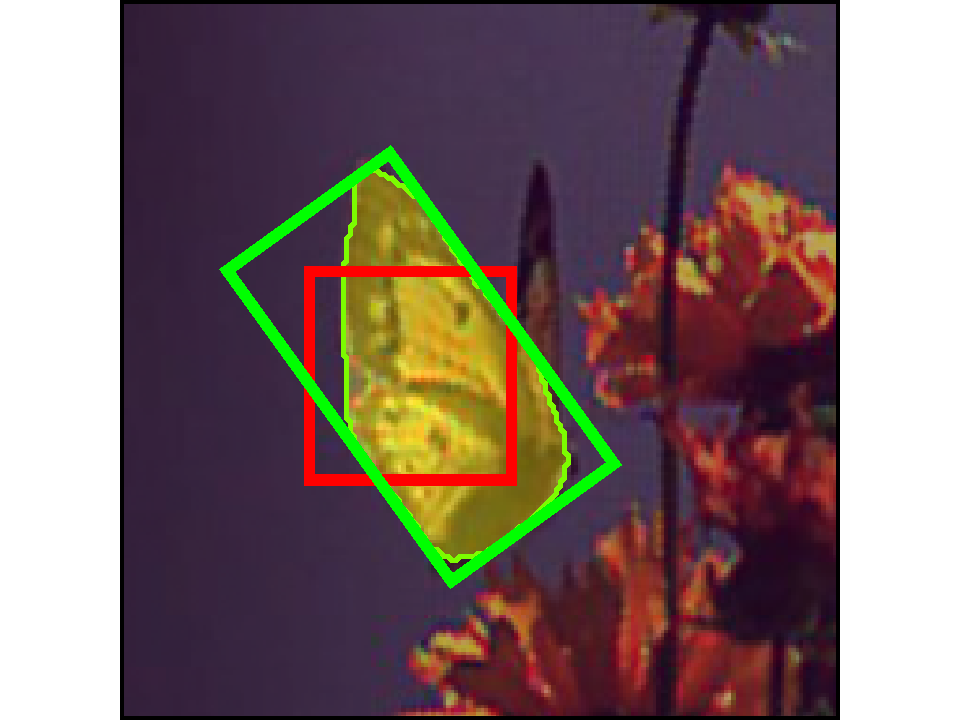
\includegraphics[trim={2cm 0cm 2cm 0cm},clip,width = 0.61in]{img/snapshots/eco_uspblackedge/03214}
\\

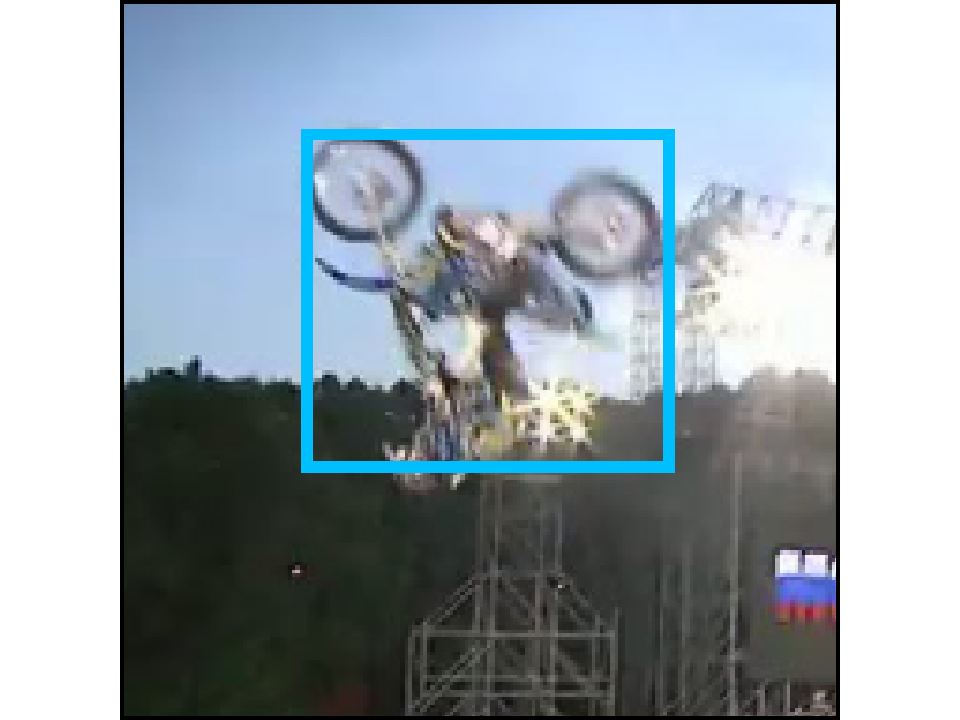
\includegraphics[trim={2cm 0cm 2cm 0cm},clip,width = 0.61in]{img/snapshots/init/00038}
&&&

&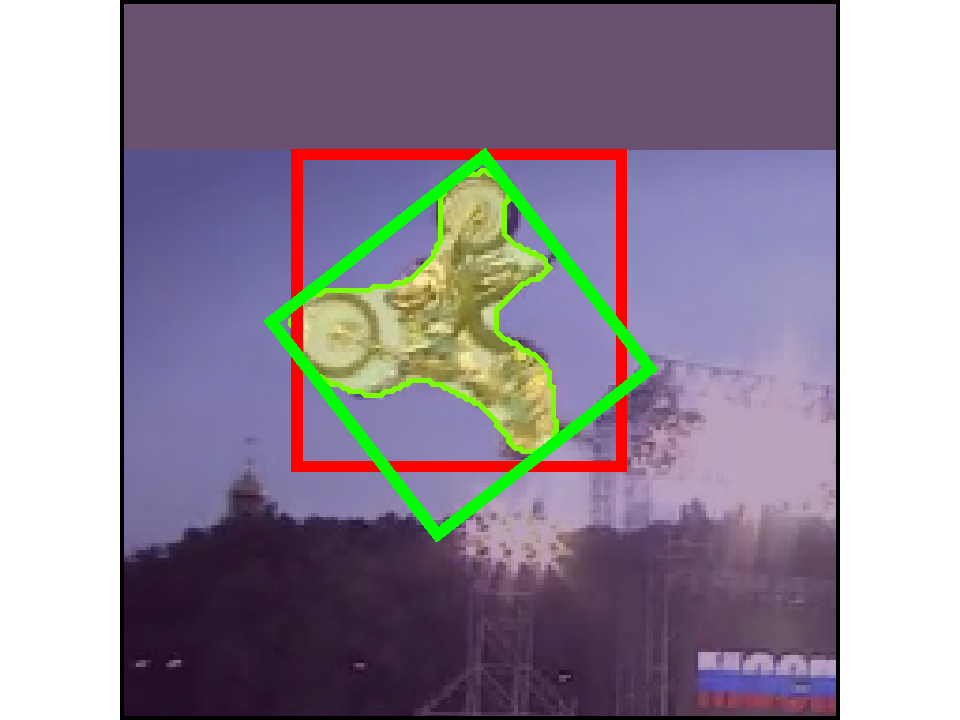
\includegraphics[trim={2cm 0cm 2cm 0cm},clip,width = 0.61in]{img/snapshots/eco_uspblackedge/14691}
& 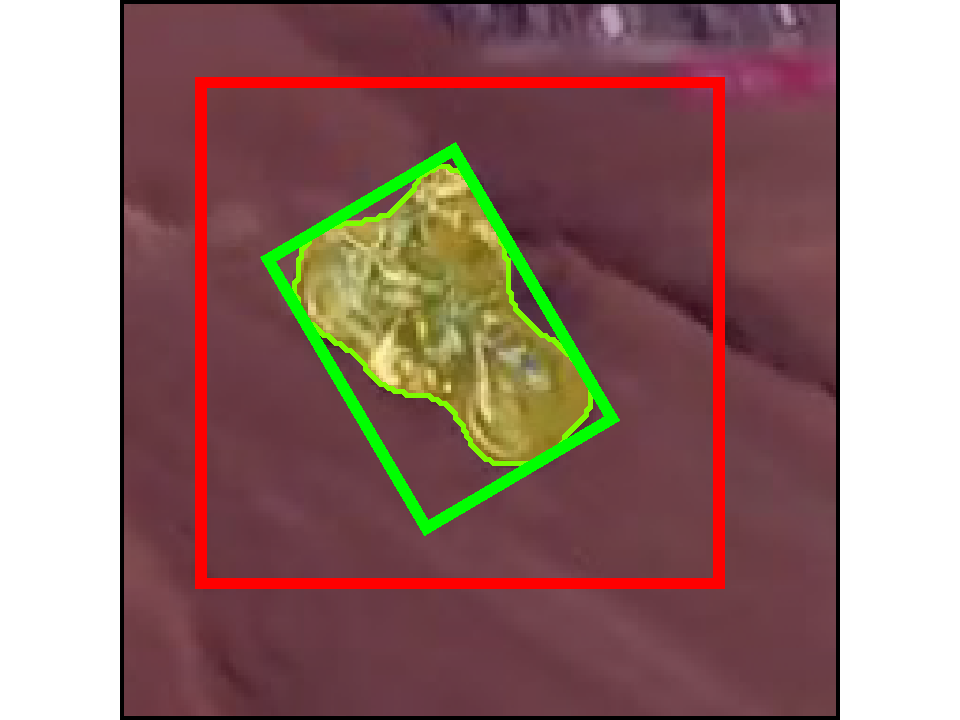
\includegraphics[trim={2cm 0cm 2cm 0cm},clip,width = 0.61in]{img/snapshots/eco_uspblackedge/14724}
& 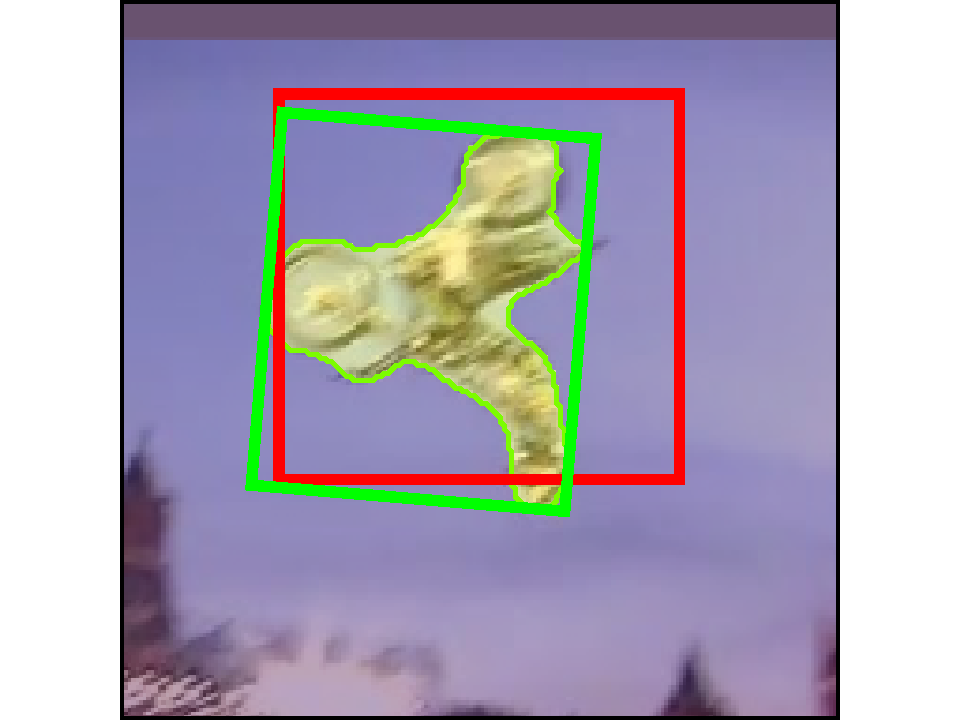
\includegraphics[trim={2cm 0cm 2cm 0cm},clip,width = 0.61in]{img/snapshots/eco_uspblackedge/14775}
& 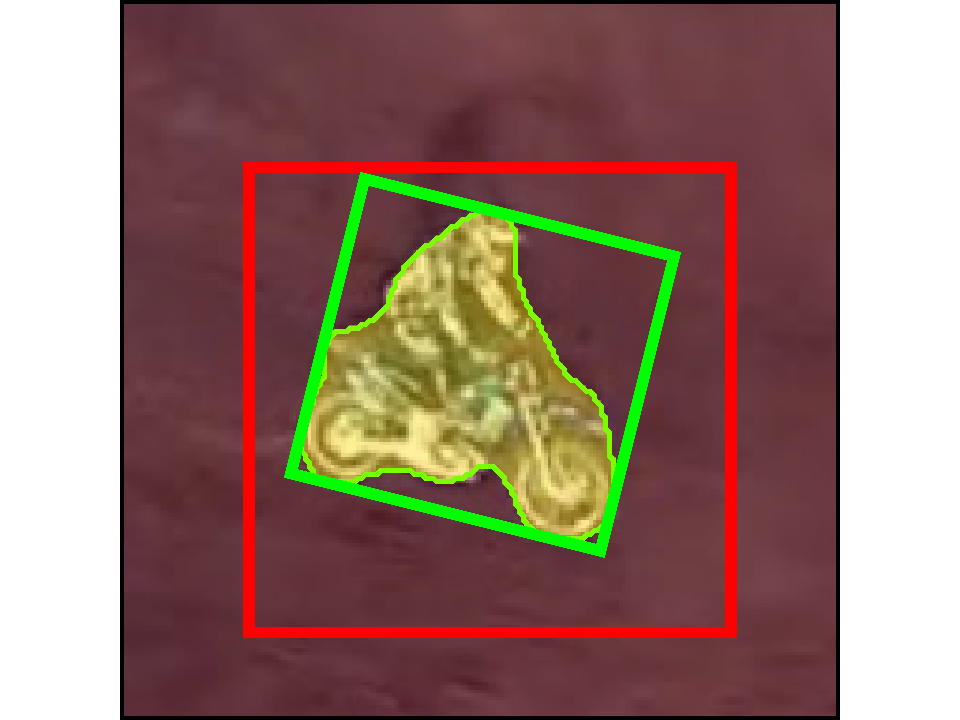
\includegraphics[trim={2cm 0cm 2cm 0cm}, clip,width = 0.61in]{img/snapshots/eco_uspblackedge/14842}

\\

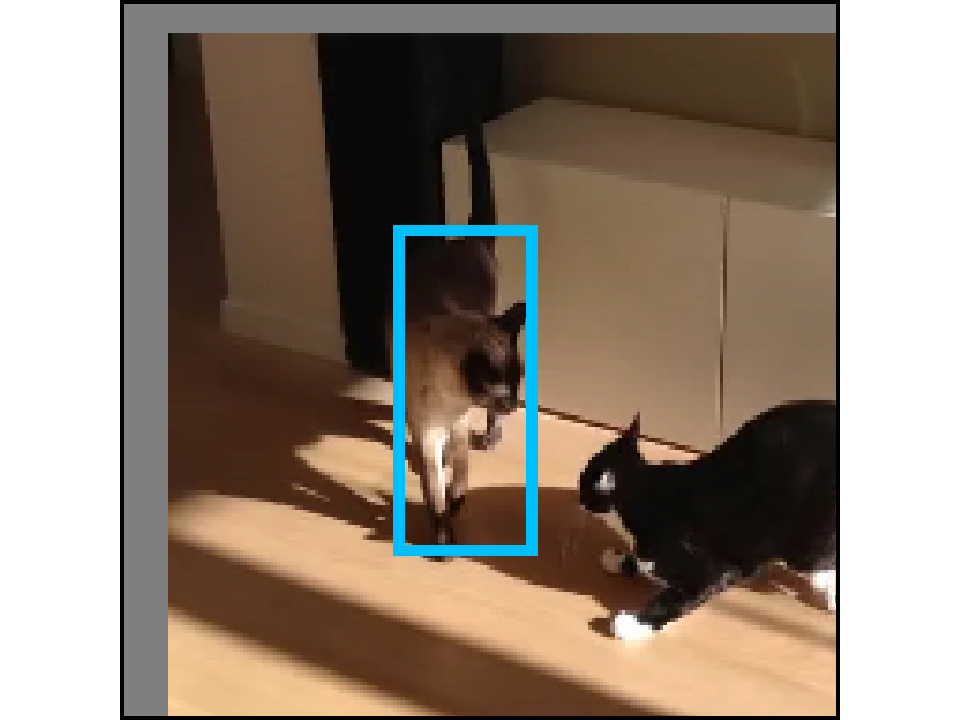
\includegraphics[trim={2cm 0cm 2cm 0cm},clip,width = 0.61in]{img/snapshots/init/00016}
&&&
&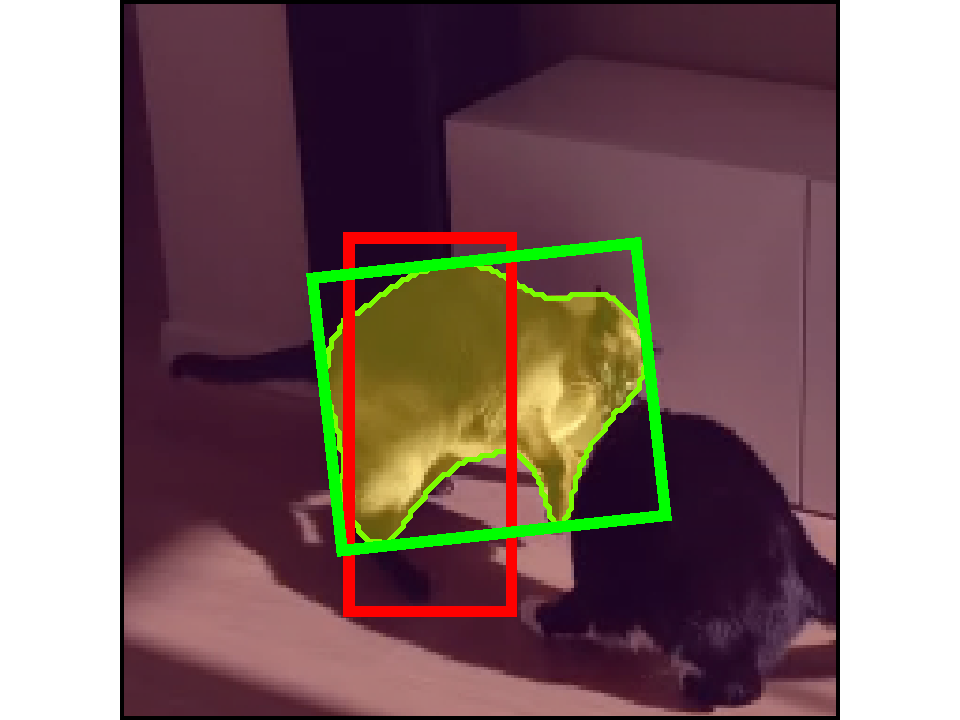
\includegraphics[trim={2cm 0cm 2cm 0cm},clip,width = 0.61in]{img/snapshots/eco_uspblackedge/04867}
& 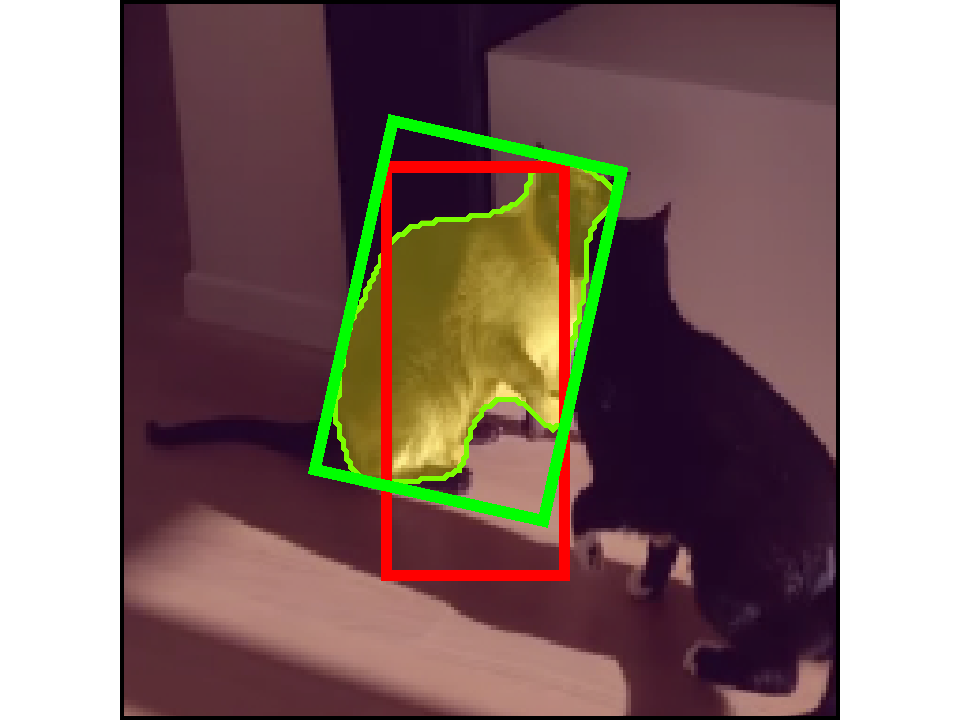
\includegraphics[trim={2cm 0cm 2cm 0cm},clip,width = 0.61in]{img/snapshots/eco_uspblackedge/04927}
& 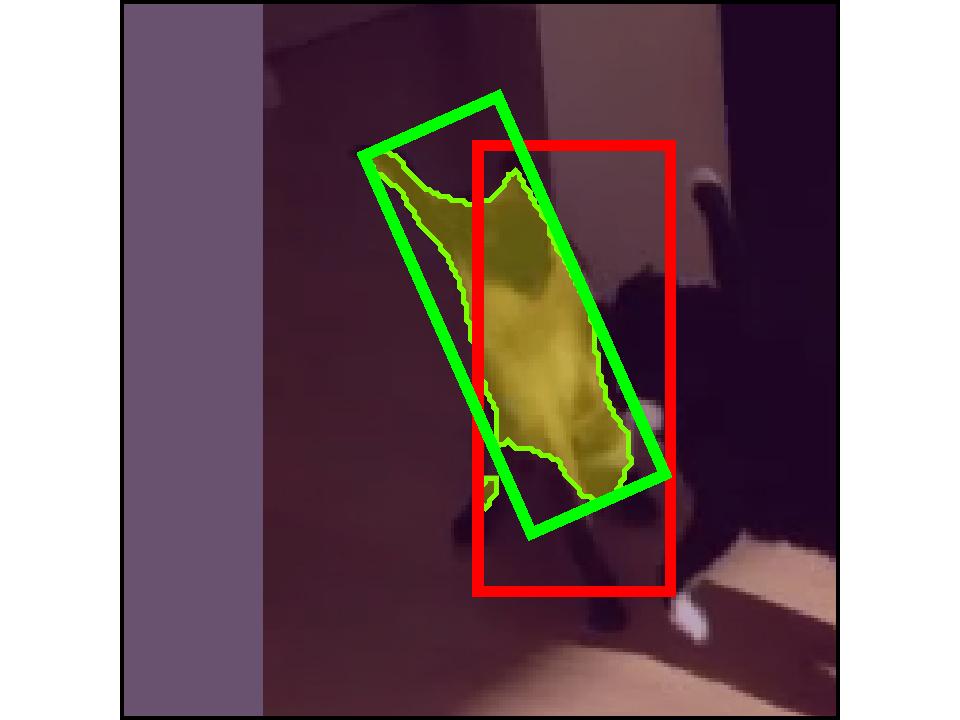
\includegraphics[trim={2cm 0cm 2cm 0cm},clip,width = 0.61in]{img/snapshots/eco_uspblackedge/04987}
& 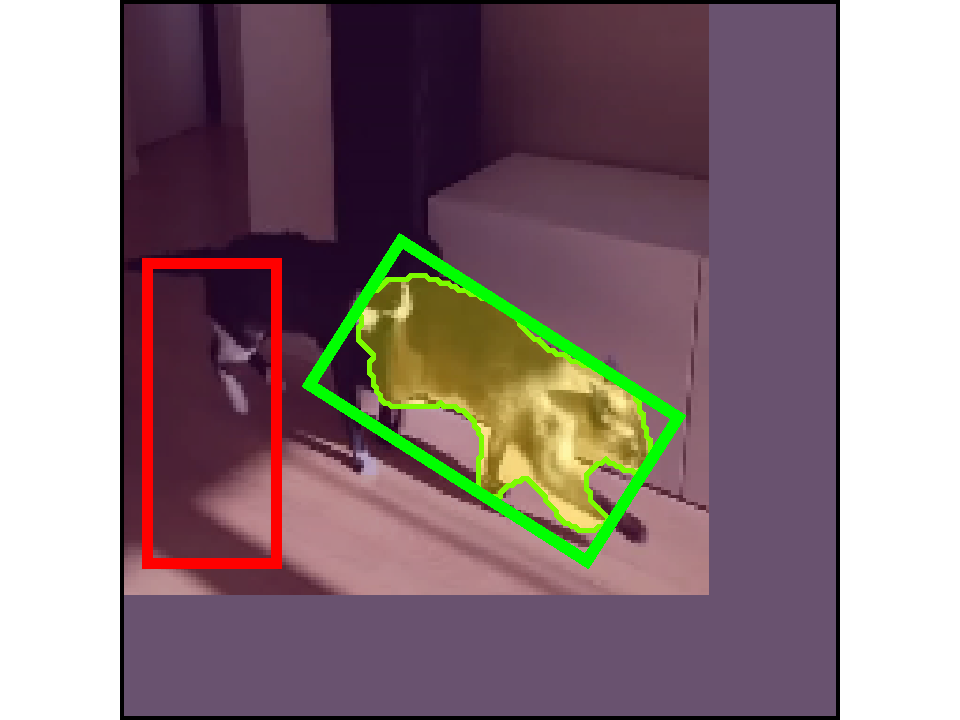
\includegraphics[trim={2cm 0cm 2cm 0cm},clip,width = 0.61in]{img/snapshots/eco_uspblackedge/05096}
\\

Init &
\multicolumn{7}{c}{Estimates}

\end{tabular}

\caption{
Our method aims at the intersection between the tasks of visual tracking and video object segmentation to achieve high practical convenience.
Like conventional object trackers, it relies on a simple bounding box initialisation (blue) and operates online.
Differently from state-of-the-art trackers such as ECO~\cite{danelljan2017eco} (red), SiamMask (green) is able to produce binary segmentation masks, which can more accurately describe the target object.
}
\label{fig:video_page1}
\vspace{-0.5cm}
\end{figure}

For many applications, it is important that tracking can be performed \emph{online}, while the video is streaming.
In other words, the tracker should not make use of future frames to reason about the current position of the object~\cite{kristan2016visual}.
This is the scenario portrayed by visual object tracking benchmarks, which represent the target object with a simple axis-aligned (\eg~\cite{wu2013online,valmadre2018long}) or rotated~\cite{kristan2016visual,VOT2018} bounding box.
Such a simple annotation helps to keep the cost of data labelling low; what is more, it allows a user to perform a quick and simple initialisation of the target.

Similar to object tracking, the task of semi-supervised \emph{video object segmentation} (VOS) requires estimating the position of an arbitrary target specified in the first frame of a video.
However, in this case the object representation consists of a binary segmentation mask which expresses whether or not a pixel belongs to the target~\cite{perazzi2016benchmark}.
Such a detailed representation is more desirable for applications that require pixel-level information, like video editing~\cite{perazzi2017video} and rotoscoping~\cite{miksik2017roam}.
Understandably, producing pixel-level estimates requires more computational resources than a simple bounding box.
As a consequence, VOS methods have been traditionally slow, often requiring several seconds per frame (\eg~\cite{wen2015jots,tsai2016video,perazzi2017learning,bao2018cnn}).
Very recently, there has been a surge of interest in faster approaches~\cite{Yang_2018_CVPR,marki2016bilateral,wug2018fast,cheng2018fast,chen2018blazingly,jampani2017video,hu2018videomatch}.
However, even the fastest still cannot operate in real-time.

In this paper, we aim at narrowing the gap between arbitrary object tracking and VOS by proposing \textit{SiamMask}, a simple multi-task learning approach that can be used to address \emph{both} problems.
Our method is motivated by the success of fast tracking approaches based on fully-convolutional Siamese networks~\cite{bertinetto2016fully} trained offline on millions of pairs of video frames (\eg \cite{SiamRPN,zhu2018distractor,he2018towards,yang2018learning}) and by the very recent availability of YouTube-VOS~\cite{xu2018youtube}, a large video dataset with pixel-wise annotations. 
We aim at retaining the offline trainability and online speed of these methods while at the same time significantly refining their representation of the target object, which is limited to a simple axis-aligned bounding box.

To achieve this goal, we simultaneously train a Siamese network on three tasks, each corresponding to a different strategy to establish correspondances between the target object and candidate regions in the new frames.
As in the fully-convolutional approach of Bertinetto \etal~\cite{bertinetto2016fully}, one task is to learn a measure of similarity between the target object and multiple candidates in a sliding window fashion.
The output is a dense response map which only indicates the location of the object, without providing any information about its spatial extent.
To refine this information, we simultaneously learn two further tasks: bounding box regression using a Region Proposal Network~\cite{ren2015faster,SiamRPN} and class-agnostic binary segmentation~\cite{DeepMask}.
Notably, binary labels are only required during offline training to compute the segmentation loss and \emph{not} online during segmentation/tracking. 
In our proposed architecture, each task is represented by a different branch departing from a shared CNN and contributes towards a final loss, which sums the three outputs together.

Once trained, SiamMask solely relies on a single bounding box initialisation, operates online without updates and produces object segmentation masks and rotated bounding boxes at 55 frames per second.
Despite its simplicity and fast speed, SiamMask establishes a new state-of-the-art on VOT-2018 for the problem of real-time object tracking.
Moreover, the \emph{same method} is also very competitive against recent semi-supervised VOS approaches on DAVIS-2016 and DAVIS-2017, while being the fastest by a large margin.
This result is achieved with a simple bounding box initialisation (as opposed to a mask) and without adopting costly techniques often used by VOS approaches such as fine-tuning~\cite{maninis2017video,perazzi2017learning,bao2018cnn,voigtlaender2017online}, data augmentation~\cite{LucidDataDreaming_CVPR17_workshops,li2018video} and optical flow~\cite{tsai2016video,bao2018cnn,perazzi2017learning,li2018video,cheng2018fast}.

The rest of this paper is organised as follows.
Section~\ref{sec:related} briefly outlines some of the most relevant prior work in visual object tracking and semi-supervised VOS; Section~\ref{sec:method} describes our proposal; Section~\ref{sec:experiments} evaluates it on four benchmarks and illustrates several ablative studies; Section~\ref{sec:conclusion} concludes the paper.
